\documentclass{article}\usepackage[]{graphicx}\usepackage[]{xcolor}
% maxwidth is the original width if it is less than linewidth
% otherwise use linewidth (to make sure the graphics do not exceed the margin)
\makeatletter
\def\maxwidth{ %
  \ifdim\Gin@nat@width>\linewidth
    \linewidth
  \else
    \Gin@nat@width
  \fi
}
\makeatother

\definecolor{fgcolor}{rgb}{0.345, 0.345, 0.345}
\newcommand{\hlnum}[1]{\textcolor[rgb]{0.686,0.059,0.569}{#1}}%
\newcommand{\hlstr}[1]{\textcolor[rgb]{0.192,0.494,0.8}{#1}}%
\newcommand{\hlcom}[1]{\textcolor[rgb]{0.678,0.584,0.686}{\textit{#1}}}%
\newcommand{\hlopt}[1]{\textcolor[rgb]{0,0,0}{#1}}%
\newcommand{\hlstd}[1]{\textcolor[rgb]{0.345,0.345,0.345}{#1}}%
\newcommand{\hlkwa}[1]{\textcolor[rgb]{0.161,0.373,0.58}{\textbf{#1}}}%
\newcommand{\hlkwb}[1]{\textcolor[rgb]{0.69,0.353,0.396}{#1}}%
\newcommand{\hlkwc}[1]{\textcolor[rgb]{0.333,0.667,0.333}{#1}}%
\newcommand{\hlkwd}[1]{\textcolor[rgb]{0.737,0.353,0.396}{\textbf{#1}}}%
\let\hlipl\hlkwb

\usepackage{framed}
\makeatletter
\newenvironment{kframe}{%
 \def\at@end@of@kframe{}%
 \ifinner\ifhmode%
  \def\at@end@of@kframe{\end{minipage}}%
  \begin{minipage}{\columnwidth}%
 \fi\fi%
 \def\FrameCommand##1{\hskip\@totalleftmargin \hskip-\fboxsep
 \colorbox{shadecolor}{##1}\hskip-\fboxsep
     % There is no \\@totalrightmargin, so:
     \hskip-\linewidth \hskip-\@totalleftmargin \hskip\columnwidth}%
 \MakeFramed {\advance\hsize-\width
   \@totalleftmargin\z@ \linewidth\hsize
   \@setminipage}}%
 {\par\unskip\endMakeFramed%
 \at@end@of@kframe}
\makeatother

\definecolor{shadecolor}{rgb}{.97, .97, .97}
\definecolor{messagecolor}{rgb}{0, 0, 0}
\definecolor{warningcolor}{rgb}{1, 0, 1}
\definecolor{errorcolor}{rgb}{1, 0, 0}
\newenvironment{knitrout}{}{} % an empty environment to be redefined in TeX

\usepackage{alltt}
\usepackage{amsmath}
\usepackage{natbib}

\newcommand{\mumolspercm}{$\mu$mols/cm$^{-3}$}
\IfFileExists{upquote.sty}{\usepackage{upquote}}{}
\begin{document}

\title{DRAFT ! Advection, Diffusion \& Reaction Modeling}
\author{Marc Los Huertos}
\date{\today~(ver. 0.4 don't read until I get to v .8!)}

\maketitle

\begin{abstract}
The movement of compounds in the environment is driven by two processes, advection and diffusion. Of course, these processes occur in three dimensions, but for this class we'll begin with one dimensional processes before getting to more complicated examples.

%\sidenote{Typeset using the Sweave function in R and \LaTeX\ using a \citet{Tufte:1983, Tufte:1997} and style.}
\end{abstract}

\section{Introduction}

Advection and diffusion are two fundamental processes that govern the transport of solutes in the environment. Advection is the process of transport of a solute by the bulk motion of the fluid. Diffusion is the process of transport of a solute by random molecular motion.

\subsection{Advection and Convection: Material and Heat}

Advection is the transport of a substance by bulk motion. Convection is the transfer of heat by the actual movement of the warmed matter. The equation that are used to describe advection and convection are similar, but the physical processes are different.

\subsection{Session Goals}

We will not become experts in advection-diffusion-reaction modeling, but we will become familiar with the processes and the equations that describe them. Moreover, we'll see a bit more about how R can be used to model these processes. After this session, I hope you can do the following:

\begin{enumerate}
	\item Describe the physical processes of advection and dispersion and reactions
	\item Describe the equations used to model A-D-R. 
	\item Analyze 1-dimensional movement using advection equations in R.
	\item Describe diffusion mathematically
	\item Analyze 1-dimensional adveecton-diffusion using R.
	\item Appreciate how two-dimensional analysis of advection-diffusion can be modeled in R.
\end{enumerate}

\subsection{The Processes and the Equations to Describe Them}


%− 1 Axξx ·( ∂ ∂xAx·(−D· ∂ξxC ∂x )− ∂ ∂x(Ax·v·ξxC)) 

\begin{equation}
- \frac{1}{A_x \xi_x} \cdot \left( \frac{\partial}{\partial x} A_x \cdot \left( -D \cdot \frac{\partial \xi_x C}{\partial x} \right) - \frac{\partial}{\partial x} \left( A_x \cdot v \cdot \xi_x C \right) \right)
\end{equation}


Here $D$ is the ``diffusion coefficient'', $v$ is the ``advection rate'', and $A_x$ and $\xi$ are the surface area and volume fraction, respectively. 

Assuming that A, $\xi$, D and v are constant along x, we can rewrite this in a more general form: 

%D∂2C ∂x2−u∂C ∂x
\begin{equation}
D \frac{\partial^2 C}{\partial x^2} - \mu \frac{\partial C}{\partial x}
\end{equation}

where $u = v/A_x \xi_x$ is the ``velocity'' of the fluid.

The movement of compounds in the environment is driven by two processes, advection and diffusion. Of course, these processes occur in three dimensions, but for this class we'll begin with one dimensional processes before getting to more complicated examples.

Nevertheless, let's look at the 3-D advection-diffusion-reacton equation in three dimensions:

\begin{equation}
\frac{\partial C}{\partial t} = \nabla \cdot (D\nabla C - \mu C) + R
\end{equation}

where $C$ is the concentration of the solute, $t$ is time, $\mu$ is the velocity of the fluid, $D$ is the diffusion coefficient, and $R$ is the reaction term.

Ok, what what is $\nabla$? It's the gradient operator, which is a vector operator that operates on a scalar function to produce a vector whose magnitude is the maximum rate of change of the function at the point of the gradient and that points in the direction of that maximum rate of change. $\nabla \cdot$ represents divergence. In this equation, $\nabla C$ represents concentration gradient.


\subsubsection{Advection}

Advection is the process of transport of a solute by the bulk motion of the fluid. The rate of advection is proportional to the velocity of the fluid and the concentration of the solute. The rate of advection is given by the equation:

\begin{equation}
\frac{\partial C}{\partial t} + \nabla \cdot (u C) = 0
\end{equation}

where $C$ is the concentration of the solute, $t$ is time, and $u$ is the velocity of the fluid. 

For one dimensional systems, the equation can be written as:

\begin{equation}
\frac{\partial C}{\partial t} + u \frac{\partial C}{\partial x} = 0
\end{equation}

where $C$ is the concentration of the solute, $t$ is time, $u$ is the velocity of the fluid, and $x$ is the spatial coordinate.

The advection equation is not simple to solve numerically: the system is a hyperbolic partial differential equation, and interest typically centers on discontinuous "shock" solutions (which are notoriously difficult for numerical schemes to handle).


\subsubsection{Diffusion}

Diffusion is the process of transport of a solute by random molecular motion. The rate of diffusion is proportional to the concentration gradient of the solute. The rate of diffusion is given by the equation:

\begin{equation}
\frac{\partial C}{\partial t} = D \nabla^2 C
\end{equation}

where $D$ is the diffusion coefficient.

\subsubsection{Advection-Diffusion Equation}

The advection-diffusion equation is a combination of the advection and diffusion equations. The advection-diffusion equation is given by the equation:

\begin{equation}
\frac{\partial C}{\partial t} + \nabla \cdot (u C) = D \nabla^2 C
\end{equation}

where $C$ is the concentration of the solute, $t$ is time, $u$ is the velocity of the fluid, and $D$ is the diffusion coefficient.

\subsubsection{Advection-Difffusion-Reaction Equation}

The advection-diffusion-reaction equation is a combination the advection, diffusion, and reaction equations. The advection-diffusion-reaction equation is given by the equation:

\begin{equation}
\frac{\partial C}{\partial t} + \nabla \cdot (u C) = D \nabla^2 C + R
\end{equation}

where $C$ is the concentration of the solute, $t$ is time, $u$ is the velocity of the fluid, $D$ is the diffusion coefficient, and $R$ is the reaction term.
  
\subsubsection{Advenction-Difffusion-Reaction in multi-phase systems and for shapes with variable geometry}

The advection-diffusion-reaction equation can be extended to multi-phase systems and to shapes with variable geometry. The advection-diffusion-reaction equation for multi-phase systems and for shapes with variable geometry is given by the equation:

\begin{equation}
\frac{\partial C}{\partial t} + \nabla \cdot (u C) = D \nabla^2 C + R
\end{equation}

where $C$ is the concentration of the solute, $t$ is time, $u$ is the velocity of the fluid, $D$ is the diffusion coefficient, and $R$ is the reaction term.

\subsection{ReacTran Package}

\citet{soetaert2017package}
  
\section{Applications using R}

\subsection{R as a Calculator and Modeling Environment}




We can use R to solve the advection-diffusion equation. The following code uses the `deSolve` package to solve the advection-diffusion equation for a simple one-dimensional case.

\begin{verbatim}
# Load the deSolve package
library(deSolve)

# Define the advection-diffusion equation
advection_diffusion <- function(t, C, parms) {
  with(as.list(parms), {
    dC <- D * (diff(C, lag = 2) - 2 * diff(C, lag = 1) + diff(C, lag = 0)) / dx^2
    dC[1] <- 0
    dC[n] <- 0
    list(dC)
  })
}

# Set the parameters
parms <- list(
  D = 0.1,  # Diffusion coefficient
  dx = 0.1  # Spatial step
)

# Set the initial conditions
C0 <- c(0, rep(0, 98), 1, rep(0, 98), 0)
  
# Set the times at which to evaluate the solution
times <- seq(0, 100, by = 1)

# Solve the advection-diffusion equation

out <- ode(y = C0, times = times, func = advection_diffusion, parms = parms)

# Plot the solution

plot(out, xlab = "Distance", ylab = "Concentration", type = "l")
\end{verbatim}

\subsection{1D Transportion Model}

The `ReacTran` package provides a function to solve the advection-diffusion-reaction equation for a simple one-dimensional case.

\begin{knitrout}
\definecolor{shadecolor}{rgb}{0.969, 0.969, 0.969}\color{fgcolor}\begin{kframe}
\begin{alltt}
\hlcom{# Load the ReacTran package}
\hlkwd{library}\hlstd{(ReacTran)}
\end{alltt}


{\ttfamily\noindent\itshape\color{messagecolor}{\#\# Loading required package: rootSolve}}

{\ttfamily\noindent\itshape\color{messagecolor}{\#\# Loading required package: deSolve}}

{\ttfamily\noindent\itshape\color{messagecolor}{\#\# Loading required package: shape}}\end{kframe}
\end{knitrout}

\begin{knitrout}
\definecolor{shadecolor}{rgb}{0.969, 0.969, 0.969}\color{fgcolor}\begin{kframe}
\begin{alltt}
\hlkwd{tran.1D}\hlstd{(}\hlkwc{C} \hlstd{=} \hlnum{1}\hlstd{,} \hlkwc{D} \hlstd{=} \hlnum{0}\hlstd{,} \hlkwc{flux.up} \hlstd{=} \hlnum{1}\hlstd{,} \hlkwc{v} \hlstd{=} \hlnum{5}\hlstd{,} \hlkwc{A}\hlstd{=} \hlnum{1}\hlstd{,} \hlkwc{dx} \hlstd{=} \hlnum{1}\hlstd{,} \hlkwc{full.output} \hlstd{=} \hlnum{TRUE}\hlstd{)}
\end{alltt}
\begin{verbatim}
## $dC
## [1] -4
## 
## $C.up
## [1] 0.2
## 
## $C.down
## [1] 1
## 
## $dif.flux
## [1] 0 0
## 
## $adv.flux
## [1] 1 5
## 
## $flux
## [1] 1 5
## 
## $flux.up
## [1] 1
## 
## $flux.down
## [1] 5
\end{verbatim}
\end{kframe}
\end{knitrout}


\subsection{Solving a 1-D reaction tranport mdodel}

\begin{knitrout}
\definecolor{shadecolor}{rgb}{0.969, 0.969, 0.969}\color{fgcolor}\begin{kframe}
\begin{alltt}
\hlkwd{library}\hlstd{(ReacTran)}
\hlstd{out} \hlkwb{<-} \hlkwd{steady.1D}\hlstd{(}\hlkwc{func} \hlstd{= advModel,} \hlkwc{y} \hlstd{=} \hlkwd{runif}\hlstd{(}\hlnum{25}\hlstd{),} \hlkwc{params} \hlstd{= parms,} \hlkwc{nspace}\hlstd{=} \hlnum{1}\hlstd{,} \hlkwc{positive} \hlstd{=} \hlnum{TRUE}\hlstd{)}
\end{alltt}
\end{kframe}
\end{knitrout}

We can use R to solve the advection-diffusion-reaction equation. The following code uses the `deSolve` package to solve the advection-diffusion-reaction equation for a simple one-dimensional case.

\begin{knitrout}
\definecolor{shadecolor}{rgb}{0.969, 0.969, 0.969}\color{fgcolor}\begin{kframe}
\begin{alltt}
\hlcom{# Load the deSolve package}
\hlkwd{library}\hlstd{(deSolve)}

\hlcom{# Define the advection-diffusion-reaction equation}
\hlstd{advection_diffusion_reaction} \hlkwb{<-} \hlkwa{function}\hlstd{(}\hlkwc{t}\hlstd{,} \hlkwc{C}\hlstd{,} \hlkwc{parms}\hlstd{) \{}
  \hlkwd{with}\hlstd{(}\hlkwd{as.list}\hlstd{(parms), \{}
    \hlstd{dC} \hlkwb{<-} \hlstd{D} \hlopt{*} \hlstd{(}\hlkwd{diff}\hlstd{(C,} \hlkwc{lag} \hlstd{=} \hlnum{2}\hlstd{)} \hlopt{-} \hlnum{2} \hlopt{*} \hlkwd{diff}\hlstd{(C,} \hlkwc{lag} \hlstd{=} \hlnum{1}\hlstd{)} \hlopt{+} \hlkwd{diff}\hlstd{(C,} \hlkwc{lag} \hlstd{=} \hlnum{0}\hlstd{))} \hlopt{/} \hlstd{dx}\hlopt{^}\hlnum{2} \hlopt{-} \hlstd{k} \hlopt{*} \hlstd{C}
    \hlstd{dC[}\hlnum{1}\hlstd{]} \hlkwb{<-} \hlnum{0}
    \hlstd{dC[n]} \hlkwb{<-} \hlnum{0}
    \hlkwd{list}\hlstd{(dC)}
  \hlstd{\})}
\hlstd{\}}

\hlcom{# Set the parameters}
\hlstd{parms} \hlkwb{<-} \hlkwd{list}\hlstd{(}
  \hlkwc{D} \hlstd{=} \hlnum{0.1}\hlstd{,}  \hlcom{# Diffusion coefficient}
  \hlkwc{dx} \hlstd{=} \hlnum{0.1}\hlstd{,}  \hlcom{# Spatial step}
  \hlkwc{k} \hlstd{=} \hlnum{0.01}  \hlcom{# Reaction rate}
\hlstd{)}

\hlcom{# Set the initial conditions}
\hlstd{C0} \hlkwb{<-} \hlkwd{c}\hlstd{(}\hlnum{0}\hlstd{,} \hlkwd{rep}\hlstd{(}\hlnum{0}\hlstd{,} \hlnum{98}\hlstd{),} \hlnum{1}\hlstd{,} \hlkwd{rep}\hlstd{(}\hlnum{0}\hlstd{,} \hlnum{98}\hlstd{),} \hlnum{0}\hlstd{)}

\hlcom{# Set the times at which to evaluate the solution}
\hlstd{times} \hlkwb{<-} \hlkwd{seq}\hlstd{(}\hlnum{0}\hlstd{,} \hlnum{100}\hlstd{,} \hlkwc{by} \hlstd{=} \hlnum{1}\hlstd{)}

\hlcom{# Solve the advection-diffusion-reaction equation}
\hlstd{out} \hlkwb{<-} \hlkwd{ode}\hlstd{(}\hlkwc{y} \hlstd{= C0,} \hlkwc{times} \hlstd{= times,} \hlkwc{func} \hlstd{= advection_diffusion_reaction,} \hlkwc{parms} \hlstd{= parms)}

\hlcom{# Plot the solution}
\hlkwd{plot}\hlstd{(out,} \hlkwc{xlab} \hlstd{=} \hlstr{"Distance"}\hlstd{,} \hlkwc{ylab} \hlstd{=} \hlstr{"Concentration"}\hlstd{,} \hlkwc{type} \hlstd{=} \hlstr{"l"}\hlstd{)}
\end{alltt}
\end{kframe}
\end{knitrout}

\subsection{1-D Reaction-Transport Model}
\begin{knitrout}
\definecolor{shadecolor}{rgb}{0.969, 0.969, 0.969}\color{fgcolor}\begin{kframe}
\begin{alltt}
\hlkwd{library}\hlstd{(ReacTran)}

\hlstd{parms} \hlkwb{<-} \hlkwd{c}\hlstd{(}\hlkwc{F0} \hlstd{=} \hlnum{1}\hlstd{,} \hlkwc{v}\hlstd{=}\hlnum{1}\hlstd{,} \hlkwc{k} \hlstd{=} \hlnum{0.1}\hlstd{,} \hlkwc{D} \hlstd{=} \hlnum{0}\hlstd{,} \hlkwc{dx} \hlstd{=} \hlnum{1}\hlstd{)}

\hlstd{advModel} \hlkwb{<-} \hlkwa{function}\hlstd{(}\hlkwc{t}\hlstd{,} \hlkwc{C}\hlstd{,} \hlkwc{parms}\hlstd{) \{}
  \hlkwd{with}\hlstd{(}\hlkwd{as.list}\hlstd{(parms), \{}
    \hlstd{Tran} \hlkwb{<-} \hlkwd{tran.1D}\hlstd{(}\hlkwc{C} \hlstd{= C,} \hlkwc{D} \hlstd{= D,} \hlkwc{flux.up} \hlstd{= F0,} \hlkwc{v} \hlstd{= v,} \hlkwc{dx} \hlstd{= dx)}
    \hlstd{Consumption} \hlkwb{=} \hlstd{k} \hlopt{*} \hlstd{C}
    \hlstd{dC} \hlkwb{<-} \hlstd{Tran}\hlopt{$}\hlstd{dC} \hlopt{-} \hlstd{Consumption}

    \hlkwd{return}\hlstd{(}\hlkwd{list}\hlstd{(}\hlkwc{dC} \hlstd{= dC,} \hlkwc{Consumption} \hlstd{= Consumption,} \hlkwc{flux.up} \hlstd{= Tran}\hlopt{$}\hlstd{flux.up,} \hlkwc{flux.down} \hlstd{= Tran}\hlopt{$}\hlstd{flux.down))}
  \hlstd{\})}
\hlstd{\}}

\hlstd{out} \hlkwb{<-} \hlkwd{steady.1D}\hlstd{(}\hlkwc{func} \hlstd{= advModel,} \hlkwc{y} \hlstd{=} \hlkwd{runif}\hlstd{(}\hlnum{25}\hlstd{),} \hlkwc{parms} \hlstd{= parms,} \hlkwc{nspec}\hlstd{=} \hlnum{1}\hlstd{,} \hlkwc{positive} \hlstd{=} \hlnum{TRUE}\hlstd{)}

\hlstd{parms} \hlkwb{<-} \hlkwd{c}\hlstd{(}\hlkwc{F0} \hlstd{=} \hlnum{1}\hlstd{,} \hlkwc{v}\hlstd{=}\hlnum{1}\hlstd{,} \hlkwc{k} \hlstd{=} \hlnum{0.5}\hlstd{,} \hlkwc{D}\hlstd{=}\hlnum{0}\hlstd{,} \hlkwc{dx} \hlstd{=} \hlnum{1}\hlstd{)}
\hlstd{out2} \hlkwb{<-} \hlkwd{steady.1D}\hlstd{(}\hlkwc{func} \hlstd{= advModel,} \hlkwc{y} \hlstd{=} \hlkwd{runif}\hlstd{(}\hlnum{25}\hlstd{),} \hlkwc{parms} \hlstd{= parms,} \hlkwc{nspec}\hlstd{=} \hlnum{1}\hlstd{,} \hlkwc{positive} \hlstd{=} \hlnum{TRUE}\hlstd{)}

\hlstd{parms} \hlkwb{<-} \hlkwd{c}\hlstd{(}\hlkwc{F0} \hlstd{=} \hlnum{1}\hlstd{,} \hlkwc{v}\hlstd{=}\hlnum{1}\hlstd{,} \hlkwc{k} \hlstd{=} \hlnum{0.5}\hlstd{,} \hlkwc{D}\hlstd{=}\hlnum{50}\hlstd{,} \hlkwc{dx} \hlstd{=} \hlnum{1}\hlstd{)}
\hlstd{out3} \hlkwb{<-} \hlkwd{steady.1D}\hlstd{(}\hlkwc{func} \hlstd{= advModel,} \hlkwc{y} \hlstd{=} \hlkwd{runif}\hlstd{(}\hlnum{25}\hlstd{),} \hlkwc{parms} \hlstd{= parms,} \hlkwc{nspec}\hlstd{=} \hlnum{1}\hlstd{,} \hlkwc{positive} \hlstd{=} \hlnum{TRUE}\hlstd{)}
\end{alltt}
\end{kframe}
\end{knitrout}

\begin{knitrout}
\definecolor{shadecolor}{rgb}{0.969, 0.969, 0.969}\color{fgcolor}\begin{kframe}
\begin{alltt}
\hlstd{out}
\end{alltt}
\begin{verbatim}
## $y
##  [1] 0.90909091 0.82644629 0.75131481 0.68301346 0.62092133 0.56447394
##  [7] 0.51315812 0.46650739 0.42409762 0.38554329 0.35049391 0.31863082
## [13] 0.28966439 0.26333126 0.23939206 0.21762914 0.19784467 0.17985879
## [19] 0.16350799 0.14864363 0.13513057 0.12284599 0.11167817 0.10152561
## [25] 0.09229601
## 
## $Consumption
##  [1] 0.090909091 0.082644629 0.075131481 0.068301346 0.062092133 0.056447394
##  [7] 0.051315812 0.046650739 0.042409762 0.038554329 0.035049391 0.031863082
## [13] 0.028966439 0.026333126 0.023939206 0.021762914 0.019784467 0.017985879
## [19] 0.016350799 0.014864363 0.013513057 0.012284599 0.011167817 0.010152561
## [25] 0.009229601
## 
## $flux.up
## [1] 1
## 
## $flux.down
## [1] 0.09229601
## 
## attr(,"precis")
## [1] 3.309670e-01 2.257957e-09
## attr(,"steady")
## [1] TRUE
## attr(,"class")
## [1] "steady1D"  "rootSolve" "list"     
## attr(,"dimens")
## [1] 25
## attr(,"nspec")
## [1] 1
\end{verbatim}
\end{kframe}
\end{knitrout}

\begin{knitrout}
\definecolor{shadecolor}{rgb}{0.969, 0.969, 0.969}\color{fgcolor}\begin{kframe}
\begin{alltt}
\hlkwd{par}\hlstd{(}\hlkwc{mfrow}\hlstd{=}\hlkwd{c}\hlstd{(}\hlnum{1}\hlstd{,}\hlnum{3}\hlstd{))}
\hlkwd{plot}\hlstd{(out,} \hlkwc{xlab} \hlstd{=} \hlstr{"X"}\hlstd{,} \hlkwc{ylab} \hlstd{=} \hlstr{"Concentration"}\hlstd{,} \hlkwc{las}\hlstd{=}\hlnum{1}\hlstd{,} \hlkwc{main}\hlstd{=}\hlstr{"Advection-Reaction: Steady State Solution"}\hlstd{)}
\end{alltt}
\end{kframe}
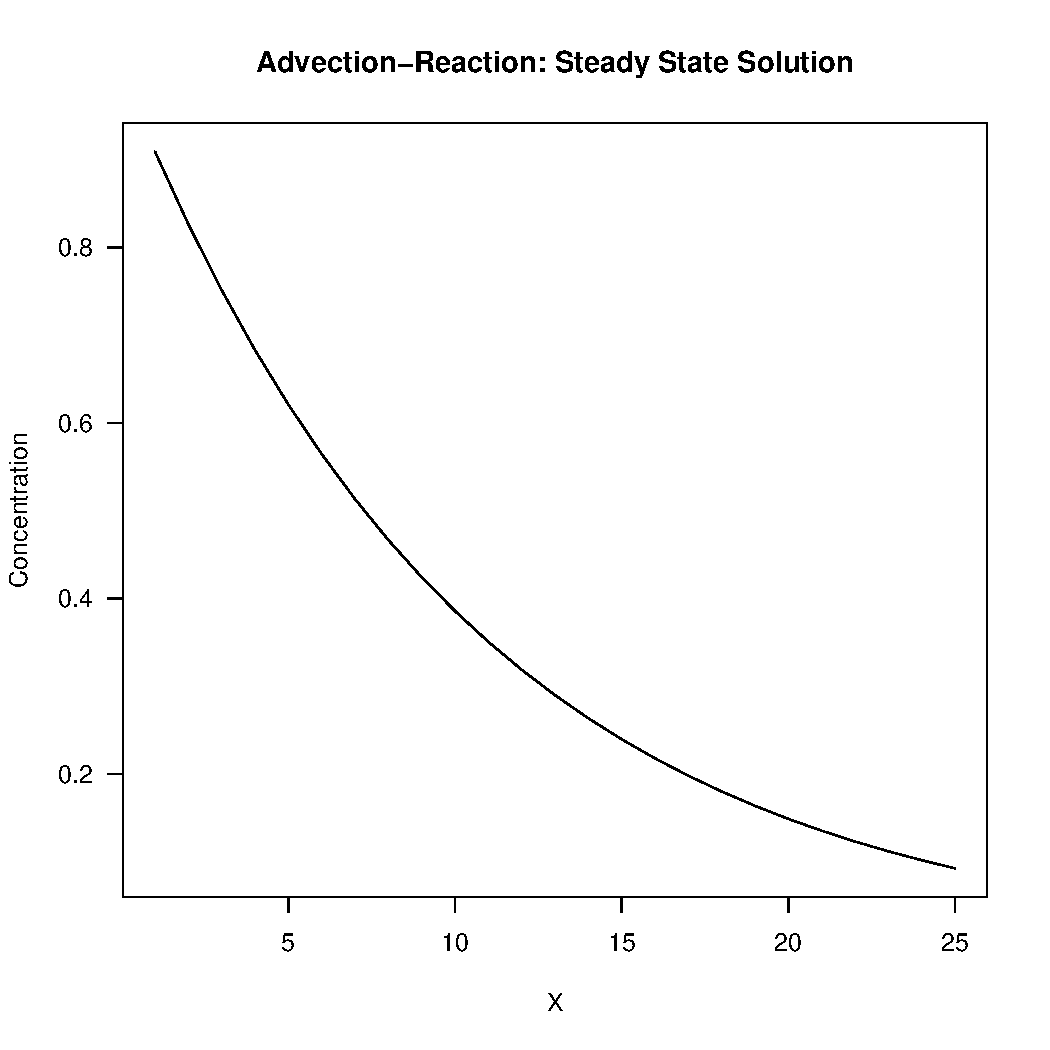
\includegraphics[width=\maxwidth]{figure/unnamed-chunk-7-1} 
\begin{kframe}\begin{alltt}
\hlkwd{plot}\hlstd{(out2,} \hlkwc{xlab} \hlstd{=} \hlstr{"X"}\hlstd{,} \hlkwc{ylab} \hlstd{=} \hlstr{"Concentration"}\hlstd{,} \hlkwc{las}\hlstd{=}\hlnum{1}\hlstd{,} \hlkwc{main}\hlstd{=}\hlstr{"Advection-Reaction: Steady State Solution"}\hlstd{)}
\end{alltt}
\end{kframe}
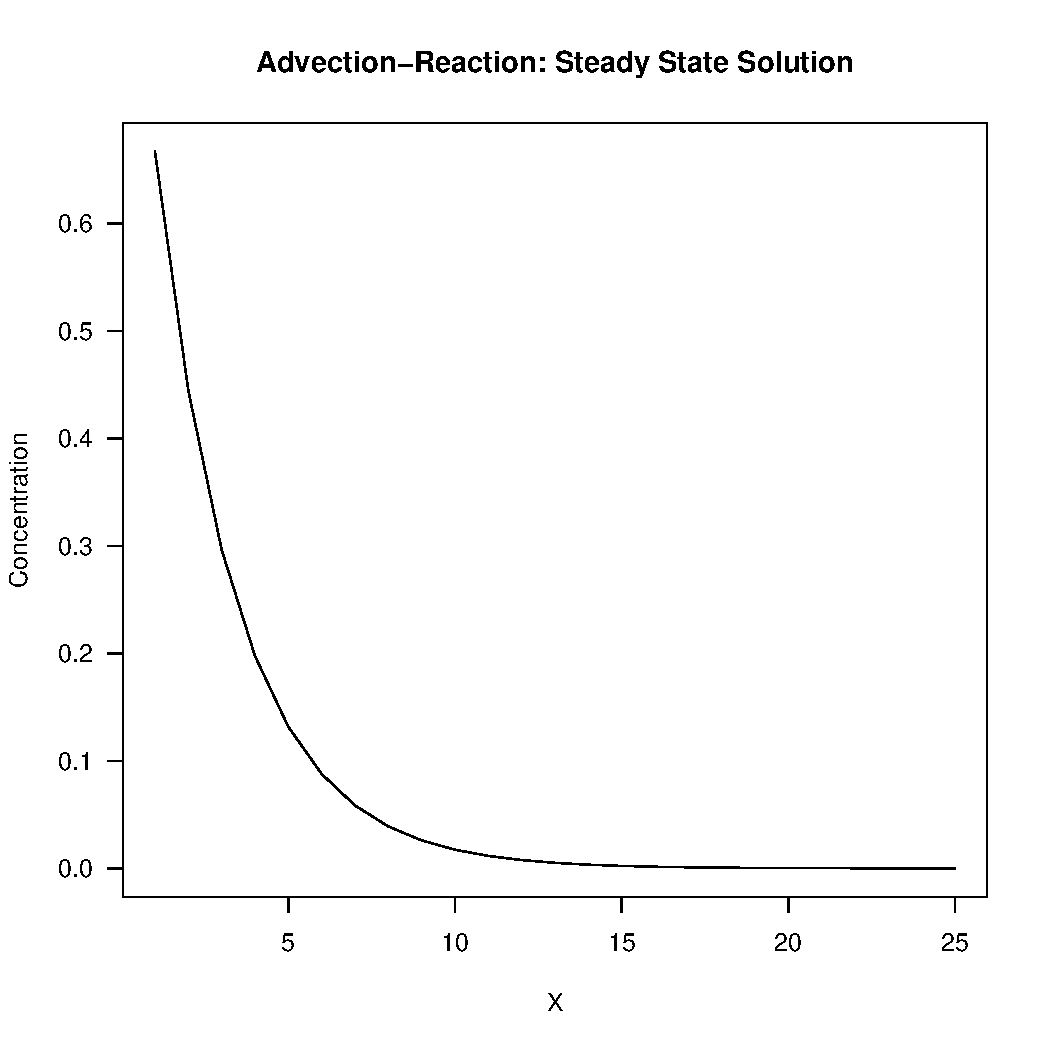
\includegraphics[width=\maxwidth]{figure/unnamed-chunk-7-2} 
\begin{kframe}\begin{alltt}
\hlkwd{plot}\hlstd{(out3,} \hlkwc{xlab} \hlstd{=} \hlstr{"X"}\hlstd{,} \hlkwc{ylab} \hlstd{=} \hlstr{"Concentration"}\hlstd{,} \hlkwc{las}\hlstd{=}\hlnum{1}\hlstd{,} \hlkwc{main}\hlstd{=}\hlstr{"Advection-Reaction: Steady State Solution"}\hlstd{)}
\end{alltt}
\end{kframe}
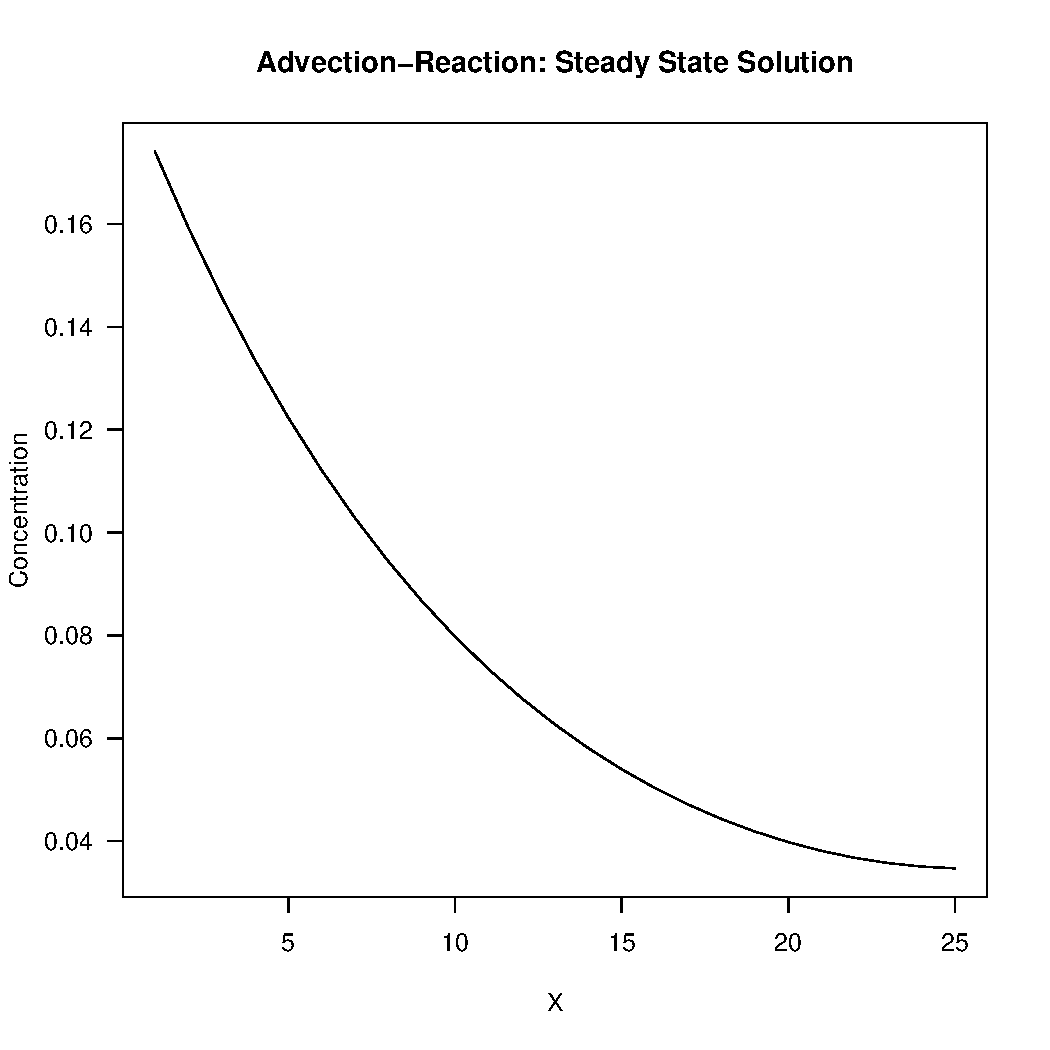
\includegraphics[width=\maxwidth]{figure/unnamed-chunk-7-3} 
\end{knitrout}

\subsection{Oxygen Consumption Porous Spherical Particle}

We will be modeling the consumption of oxygen in a "sand-sized" porous spherical particle. The model is based on the following equation:

\[ \frac{\partial C}{\partial t} = -v \frac{\partial C}{\partial x} - k(C) \]

where \( C \) is the concentration of oxygen, \( D \) is the diffusion coefficient, \( v \) is the velocity of the fluid, and \( k(C) \) is the rate of oxygen consumption.

At this scale the velocity will be zero. Thus, we will rely on diffusion to for the oxygen movement to where it is consumed. 



We start with defining the size and porosity of the particle and use R to create a grid to solve the advection-diffusion-reaction equation.

\begin{table}[h]
\caption{Chararacteristics of the Particle}
\centering
\begin{tabular}{|l|l|c|c|} \hline
Parameter & Description & Typical Range &  Modelled Value \\ \hline\hline
\( R \) & Radius of the particle & \( 0.005 - 0.2 \) cm &  0.025 cm \\
Porosity & Proportion of void space & \(0.005 -- 0.7\) &  0.7 \\ \hline
\end{tabular}
\end{table}

We will create a grid to model the particle with Radius \( R \) and \( N \) (= 100) grid points. We will also define the properties of the particle such as porosity, diffusion coefficient (D = 400), and the rate of oxygen consumption, R$_{02}$ = \ensuremath{10^{6}}.

Although we are modeling a one-dimensional system, we will need to create a grid surface as a circle to effectively model the particle surface area changes as O2 diffuses into the particle and is consumed by the reactions in the particle.

\begin{knitrout}
\definecolor{shadecolor}{rgb}{0.969, 0.969, 0.969}\color{fgcolor}\begin{kframe}
\begin{alltt}
\hlstd{grid} \hlkwb{<-} \hlkwd{setup.grid.1D}\hlstd{(}\hlkwc{x.up}\hlstd{=}\hlnum{0}\hlstd{,} \hlkwc{L} \hlstd{= R,} \hlkwc{N} \hlstd{= N)}

\hlstd{por.grid} \hlkwb{<-} \hlkwd{setup.prop.1D}\hlstd{(}\hlkwc{value}\hlstd{=por,} \hlkwc{grid}\hlstd{=grid)}
\hlstd{D.grid} \hlkwb{<-} \hlkwd{setup.prop.1D}\hlstd{(}\hlkwc{value}\hlstd{=D,} \hlkwc{grid}\hlstd{=grid)}

\hlstd{sphere.surf} \hlkwb{<-} \hlkwa{function}\hlstd{(}\hlkwc{x}\hlstd{)} \hlnum{4}\hlopt{*}\hlstd{pi}\hlopt{*}\hlstd{x}\hlopt{^}\hlnum{2}
\hlstd{A.grid} \hlkwb{<-} \hlkwd{setup.prop.1D}\hlstd{(}\hlkwc{func}\hlstd{=sphere.surf,}  \hlkwc{grid}\hlstd{=grid)}
\end{alltt}
\end{kframe}
\end{knitrout}

Finally, we need to define the O2 concentration at the surface of the particle and the O2 consumption rate of the particle. 

\begin{table}[h]
\caption{Oxygen Consumption in the Particle}
\centering
\begin{tabular}{|l|l|c|c|} \hline
Parameter & Description & Typical Range &  Modelled Value \\ \hline\hline
\( C_{ow} \) & Concentration of O2 in Water & \( 0.1 - 0.3 \) \mumolspercm &  0.25 \mumolspercm \\
\( R_{02} \) & Rate of oxygen consumption & \( 10^5 - 10^6 \) \mumolspercm~/year &  \ensuremath{10^{6}} \mumolspercm/year \\
\( K_s \) & O2 saturation & \( 0.001 - 0.01 \) \mumolspercm &  0.005 \mumolspercm \\ \hline
\end{tabular}
\end{table}

Note, we often measure oxygen using ppm (parts per million), but the model uses \mumolspercm. The conversion is 1 ppm = 0.0224 \mumolspercm, thus, we are modeling \(Ks \) within a range of 2.24 - 6.72 ppm, using Ks = 0.22 \mumolspercm.


Next we create a function to model the oxygen consumption in the, particle that relies on We will use the \texttt{tran.1D} function to solve the advection-diffusion equation and the \texttt{steady.1D} function to solve the steady state solution of the advection-diffusion-reaction equation.

\begin{knitrout}
\definecolor{shadecolor}{rgb}{0.969, 0.969, 0.969}\color{fgcolor}\begin{kframe}
\begin{alltt}
\hlstd{Aggregate.Model} \hlkwb{<-} \hlkwa{function}\hlstd{(}\hlkwc{time}\hlstd{,} \hlkwc{O2}\hlstd{,} \hlkwc{pars}\hlstd{) \{}
  \hlstd{tran} \hlkwb{<-} \hlkwd{tran.1D}\hlstd{(}\hlkwc{C} \hlstd{= O2,} \hlkwc{C.down} \hlstd{= C.ow.02,} \hlkwc{D} \hlstd{= D.grid,}
          \hlkwc{A}\hlstd{=A.grid,} \hlkwc{VF} \hlstd{= por.grid,} \hlkwc{dx} \hlstd{= grid)}
    \hlstd{reac} \hlkwb{<-} \hlopt{-} \hlstd{R.02} \hlopt{*} \hlstd{(O2} \hlopt{/}\hlstd{(Ks} \hlopt{+} \hlstd{O2))}
    \hlkwd{return}\hlstd{(}\hlkwd{list}\hlstd{(}\hlkwc{dCdt}\hlstd{= tran}\hlopt{$}\hlstd{dC} \hlopt{+} \hlstd{reac,} \hlkwc{reac} \hlstd{= reac,}
                \hlkwc{flux.up}\hlstd{=tran}\hlopt{$}\hlstd{flux.up,} \hlkwc{flux.down}\hlstd{=tran}\hlopt{$}\hlstd{flux.down))}
\hlstd{\}}


\hlstd{O2.agg} \hlkwb{<-} \hlkwd{steady.1D}\hlstd{(}\hlkwc{y} \hlstd{=} \hlkwd{runif}\hlstd{(N),} \hlkwc{func}\hlstd{=Aggregate.Model,}
                    \hlkwc{nspec}\hlstd{=}\hlnum{1}\hlstd{,} \hlkwc{positive}\hlstd{=}\hlnum{TRUE}\hlstd{,} \hlkwc{atol} \hlstd{=} \hlnum{1e-10}\hlstd{)}
\end{alltt}
\end{kframe}
\end{knitrout}


\begin{figure}[h]
\centering
\caption{Oxygen Consumption in a Porous Sphere}
\begin{knitrout}
\definecolor{shadecolor}{rgb}{0.969, 0.969, 0.969}\color{fgcolor}
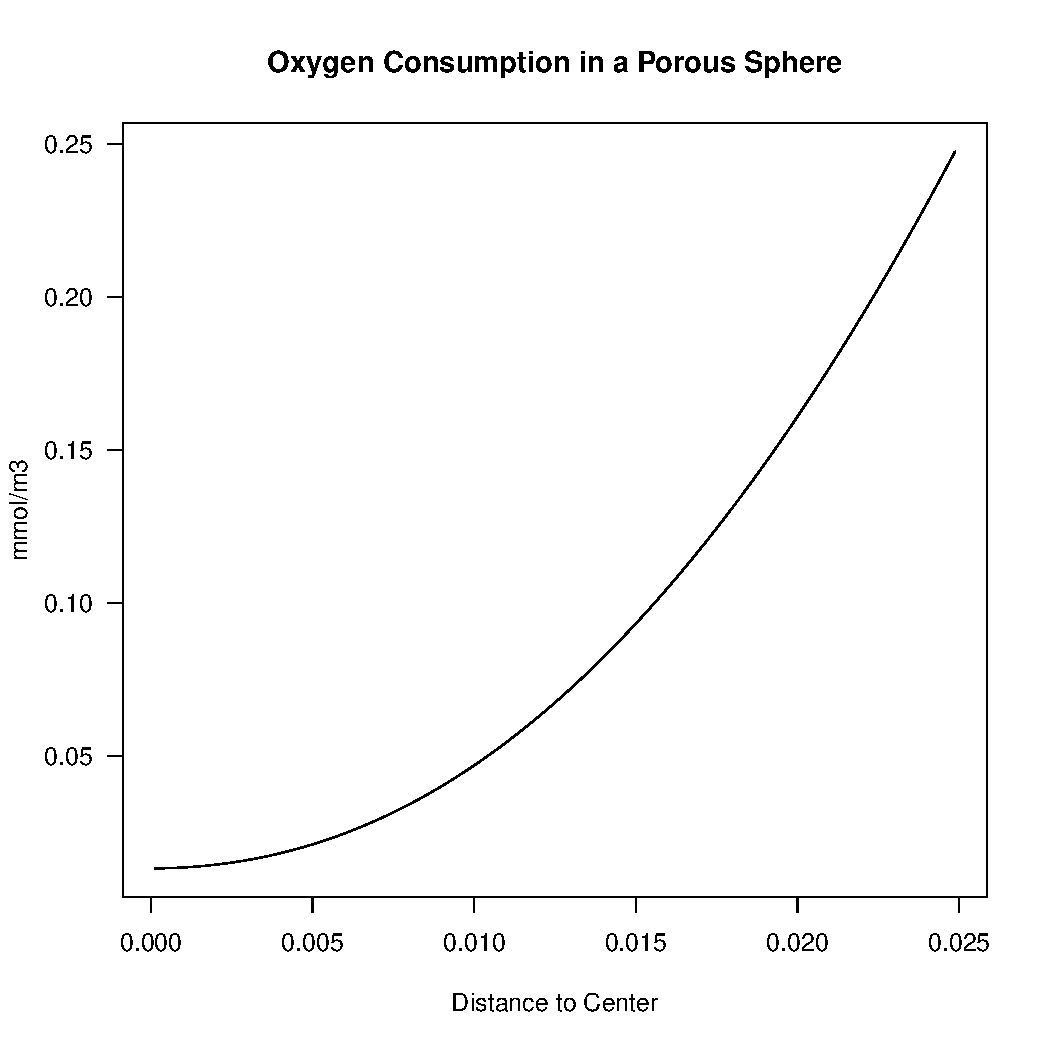
\includegraphics[width=\maxwidth]{figure/plotO2agg-1} 
\end{knitrout}
\end{figure}

The plot shows the oxygen concentration in the particle. The concentration is highest at the surface and decreases as it moves into the particle. The concentration is zero at the center of the particle.

\begin{figure}[h]
\begin{knitrout}
\definecolor{shadecolor}{rgb}{0.969, 0.969, 0.969}\color{fgcolor}
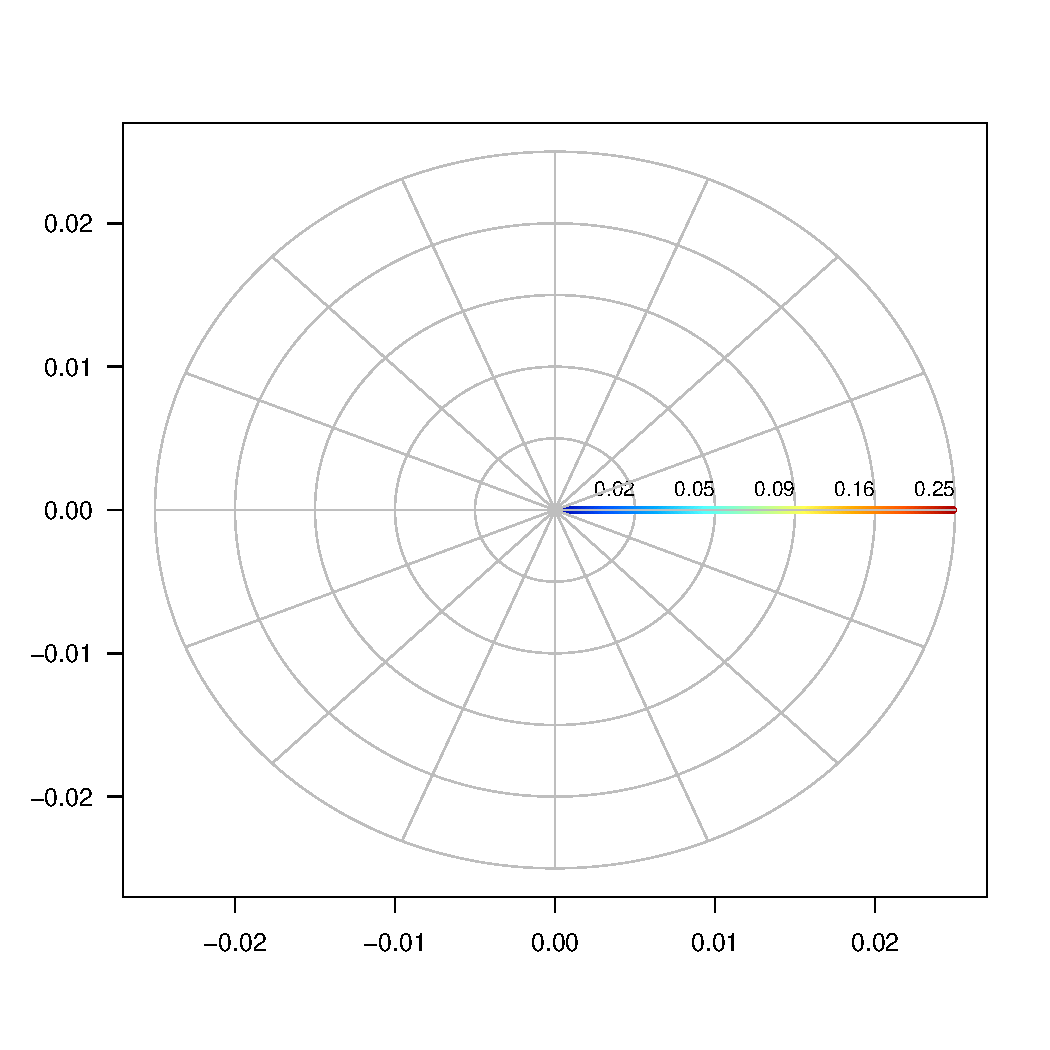
\includegraphics[width=\maxwidth]{figure/circleplot-1} 
\end{knitrout}
\end{figure}







%\printclassoptions

% Setting up the margins, etc for R





\begin{knitrout}
\definecolor{shadecolor}{rgb}{0.969, 0.969, 0.969}\color{fgcolor}\begin{kframe}
\begin{alltt}
\hlstd{diffusion2D} \hlkwb{<-} \hlkwa{function}\hlstd{(}\hlkwc{t}\hlstd{,}\hlkwc{conc}\hlstd{,}\hlkwc{par}\hlstd{)\{}
\hlstd{Conc} \hlkwb{<-} \hlkwd{matrix}\hlstd{(}\hlkwc{nr}\hlstd{=n,}\hlkwc{nc}\hlstd{=n,}\hlkwc{data}\hlstd{=conc)} \hlcom{# vector to 2-D matrix}
\hlstd{dConc} \hlkwb{<-} \hlopt{-}\hlstd{r}\hlopt{*}\hlstd{Conc}\hlopt{*}\hlstd{Conc} \hlcom{# consumption}
\hlstd{BND} \hlkwb{<-} \hlkwd{rep}\hlstd{(}\hlnum{1}\hlstd{,n)} \hlcom{# boundary concentration}

\hlcom{# constant production in certain cells}
\hlstd{dConc[ii]}\hlkwb{<-} \hlstd{dConc[ii]}\hlopt{+} \hlstd{p}

\hlcom{#diffusion in X-direction; boundaries=imposed concentration}

\hlstd{Flux} \hlkwb{<-} \hlopt{-}\hlstd{Dx} \hlopt{*} \hlkwd{rbind}\hlstd{(}\hlkwd{rep}\hlstd{(}\hlnum{0}\hlstd{,n),(Conc[}\hlnum{2}\hlopt{:}\hlstd{n,]}\hlopt{-}\hlstd{Conc[}\hlnum{1}\hlopt{:}\hlstd{(n}\hlopt{-}\hlnum{1}\hlstd{),]),}\hlkwd{rep}\hlstd{(}\hlnum{0}\hlstd{,n))}\hlopt{/}\hlstd{dx}
\hlstd{dConc} \hlkwb{<-} \hlstd{dConc} \hlopt{-} \hlstd{(Flux[}\hlnum{2}\hlopt{:}\hlstd{(n}\hlopt{+}\hlnum{1}\hlstd{),]}\hlopt{-}\hlstd{Flux[}\hlnum{1}\hlopt{:}\hlstd{n,])}\hlopt{/}\hlstd{dx}

\hlcom{#diffusion in Y-direction}
\hlstd{Flux} \hlkwb{<-} \hlopt{-}\hlstd{Dy} \hlopt{*} \hlkwd{cbind}\hlstd{(}\hlkwd{rep}\hlstd{(}\hlnum{0}\hlstd{,n),(Conc[,}\hlnum{2}\hlopt{:}\hlstd{n]}\hlopt{-}\hlstd{Conc[,}\hlnum{1}\hlopt{:}\hlstd{(n}\hlopt{-}\hlnum{1}\hlstd{)]),}\hlkwd{rep}\hlstd{(}\hlnum{0}\hlstd{,n))}\hlopt{/}\hlstd{dy}
\hlstd{dConc} \hlkwb{<-} \hlstd{dConc} \hlopt{-} \hlstd{(Flux[,}\hlnum{2}\hlopt{:}\hlstd{(n}\hlopt{+}\hlnum{1}\hlstd{)]}\hlopt{-}\hlstd{Flux[,}\hlnum{1}\hlopt{:}\hlstd{n])}\hlopt{/}\hlstd{dy}

\hlkwd{return}\hlstd{(}\hlkwd{list}\hlstd{(}\hlkwd{as.vector}\hlstd{(dConc)))}
\hlstd{\}}
\end{alltt}
\end{kframe}
\end{knitrout}

After specifying the values of the parameters, 10 cells on the 2-D grid where there will be
substance produced are randomly selected (ii).

14 Package rootSolve : roots, gradients and steady-states in R
0.0 0.2 0.4 0.6 0.8 1.0
0.0 0.2 0.4 0.6 0.8 1.0
2-D diffusion+production
x
y
Figure 5: Steady-state solution of the nonlinear 2-Dimensional model
\begin{knitrout}
\definecolor{shadecolor}{rgb}{0.969, 0.969, 0.969}\color{fgcolor}\begin{kframe}
\begin{alltt}
\hlcom{# parameters}
\hlstd{dy} \hlkwb{<-} \hlstd{dx} \hlkwb{<-} \hlnum{1} \hlcom{# grid size}
\hlstd{Dy} \hlkwb{<-} \hlstd{Dx} \hlkwb{<-} \hlnum{1.5} \hlcom{# diffusion coeff, X- and Y-direction}
\hlstd{r} \hlkwb{<-} \hlnum{0.01} \hlcom{# 2-nd-order consumption rate (/time)}
\hlstd{p} \hlkwb{<-} \hlnum{20} \hlcom{# 0-th order production rate (CONC/t)}
\hlstd{n} \hlkwb{<-} \hlnum{100}
\hlcom{# 10 random cells where substance is produced at rate p}
\hlstd{ii} \hlkwb{<-} \hlkwd{trunc}\hlstd{(}\hlkwd{cbind}\hlstd{(}\hlkwd{runif}\hlstd{(}\hlnum{10}\hlstd{)}\hlopt{*}\hlstd{n}\hlopt{+}\hlnum{1}\hlstd{,}\hlkwd{runif}\hlstd{(}\hlnum{10}\hlstd{)}\hlopt{*}\hlstd{n}\hlopt{+}\hlnum{1}\hlstd{))}
\end{alltt}
\end{kframe}
\end{knitrout}
The steady-state is found using function steady.2D. It takes as arguments a.o. the dimensionality
of the problem (dimens) and lrw=1000000, the length of the work array needed by
the solver. If this value is set too small, the solver will return with the size needed.
It takes about 0.5 second to solve this 10000 state variable model.
\begin{knitrout}
\definecolor{shadecolor}{rgb}{0.969, 0.969, 0.969}\color{fgcolor}\begin{kframe}
\begin{alltt}
\hlstd{Conc0} \hlkwb{<-} \hlkwd{matrix}\hlstd{(}\hlkwc{nr}\hlstd{=n,}\hlkwc{nc}\hlstd{=n,}\hlnum{10.}\hlstd{)}
\hlkwd{print}\hlstd{(}\hlkwd{system.time}\hlstd{(}
\hlstd{ST3} \hlkwb{<-} \hlkwd{steady.2D}\hlstd{(Conc0,}\hlkwc{func}\hlstd{=diffusion2D,}\hlkwc{parms}\hlstd{=}\hlkwa{NULL}\hlstd{,}\hlkwc{pos}\hlstd{=}\hlnum{TRUE}\hlstd{,}\hlkwc{dimens}\hlstd{=}\hlkwd{c}\hlstd{(n,n),}
\hlkwc{lrw}\hlstd{=}\hlnum{1000000}\hlstd{,}\hlkwc{atol}\hlstd{=}\hlnum{1e-10}\hlstd{,}\hlkwc{rtol}\hlstd{=}\hlnum{1e-10}\hlstd{,}\hlkwc{ctol}\hlstd{=}\hlnum{1e-10}\hlstd{)}
\hlstd{))}
\end{alltt}
\begin{verbatim}
##    user  system elapsed 
##   0.242   0.022   0.265
\end{verbatim}
\end{kframe}
\end{knitrout}
user system elapsed
1.044 0.032 1.076
The S3 image method is used to generate the steady-state plot.

\begin{knitrout}
\definecolor{shadecolor}{rgb}{0.969, 0.969, 0.969}\color{fgcolor}\begin{kframe}
\begin{alltt}
\hlkwd{image}\hlstd{(ST3,}\hlkwc{main}\hlstd{=}\hlstr{"2-D diffusion+production"}\hlstd{,} \hlkwc{xlab}\hlstd{=}\hlstr{"x"}\hlstd{,} \hlkwc{ylab}\hlstd{=}\hlstr{"y"}\hlstd{)}
\end{alltt}
\end{kframe}
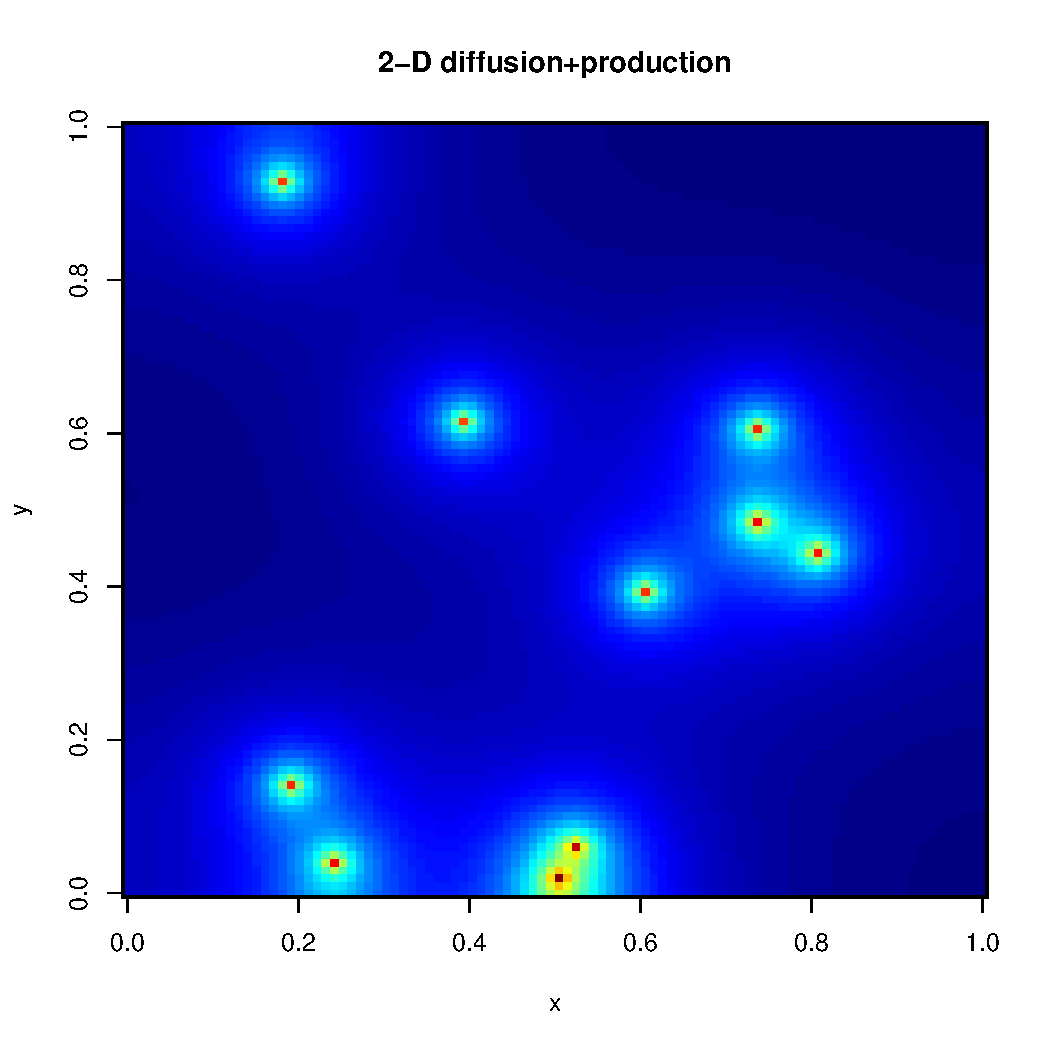
\includegraphics[width=\maxwidth]{figure/unnamed-chunk-15-1} 
\end{knitrout}


\section{Considering 2D Models}

2.4. Steady-state solution of 2-D PDEs
Function steady.2D effciently snds the steady-state of 2-dimensional problems.
Karline Soetaert 13
In the following model
@C
@t
= Dx 
@2C
@x2 + Dy 
@2C
@y2
.. r  C2 + pxy
a substance C is consumed at a quadratic rate (r C2), while dispersing in X- and Y-direction.
At certain positions (x,y) the substance is produced (rate p).
The model is solved on a square (100*100) grid. There are zero-
ux boundary conditions at
the 4 boundaries.
The term Dx  @2C
@x2 is in fact shorthand for:
..
@Flux
@x
where
Flux = ..Dx 
@C
@x
i.e. it is the negative of the 
ux gradient, where the 
ux is due to diffusion.
In the numerical approximation fo the 
ux, the concentration gradient is approximated as the
subtraction of two matrices, with the columns or rows shifted (e.g. Conc[2:n,]-Conc[1:(n-1),]).
The 
ux gradient is then also approximated by subtracting entire matrices
(e.g. Flux[2:(n+1),]-Flux[1:(n),]). This is very fast. The zero-
ux at the boundaries is
imposed by binding a column or row with 0-s.

\section{Conclusion}


% bibiliography section here-------------------------------------------
%\clearpage

\bibliographystyle{apalike}
%\renewcommand\bibname{References}{}
\bibliography{/home/mwl04747/RTricks/references}%	\addcontentsline{toc}{chapter}{References}




\end{document}
